\section{Moving Reconstructions}
\label{sec:moving}

\subsection{Purpose}
The TR process assumes that the environment remains fixed between the time-forward and time-reversed steps. It also assumes that the source and target remain fixed between these two steps. However, in a practical WPT system it is desirable to support a receiver in motion. This ability gives a convenient benefit to the consumer, who would not be limited to keeping their mobile device stationary for charging. This is a gap in the current market, which TR may be able to fill. In this section, we propose and investigate a method for using the broad spatial voltage profile to provide a consistent voltage to a receiver in motion.

The experiment is conducted in two parts: mapping the spatial voltage profile of a TR reconstructed signal, and iteratively updating the target location of the time reversal mirror. The first part of the experiment intends to consider the extent to which a reconstruction is localized in space. This property has implications for several parts of the WPT scheme including system efficiency, health concerns, and tolerance in receiver position relative to the target location. A broad reconstruction in space would relate to a lower efficiency, because only a fraction of the energy that is being sent is collected by the receiver. Consequently, if the reconstruction is broad then there is a possibility that some energy could be sent to an unintended nearby medium; for example, the target device might be in a user's pocket, and a broad profile could indicate that the user themself would be absorbing some of that energy. While both of these effects are generally things that we would like to avoid in a WPT system, it also could facilitate the accommodation of a moving receiver. A profile that is not particularly localized would allow the receiver to shift slightly from the target location and still collect a significant portion of the energy packet that was sent. When the voltage level at the receiver's position drops below some acceptable level, the TR process could be performed again. This would update the target location to the receiver's current location, and reset the voltage at the receiver to the peak value of the reconstruction. A broader reconstruction in space would allow this process to be performed less frequently, while a narrower reconstruction may greatly limit the speed that the receiver could travel at.

\subsection{Spatial Profiling}
\label{sec:spatial-profile}
\subsubsection{Methodology}

The setting for this experiment differs only slightly from the one described in Section~\ref{sec:ltr-meth}: now, the receiving antenna is mounted on a PI MikroMove \texttt{M-415.DG} translation stage, shown in Figure~\ref{fig:mikro-move}, which allows the cavity to remain sealed during translation.  Initially, the receiver is moved to the middle of the scanning range (denoted position 0). An interrogation pulse is used to capture a sona and begin creating reconstructions at this initial position. The receiver is then moved from the bottom (-35~mm) to the top (+35~mm) of the scanning range, stopping every 0.2~mm to measure and record the \ptp{} voltage of the reconstruction (still focused on 0) at each point.

\begin{figure}[h!]
\centering
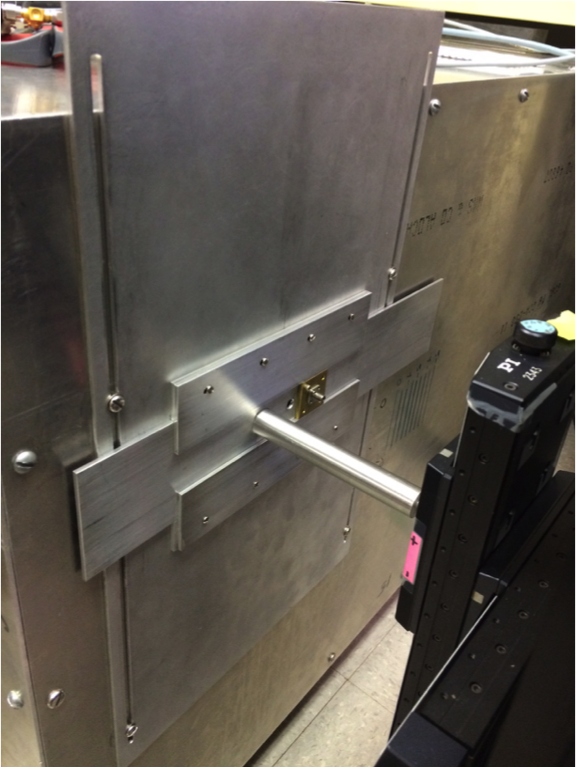
\includegraphics[width=0.75\textwidth]{moving/mikro-move-1}
    \caption[MikroMove Translation Stage]{The PI MikroMove translation stage (black, right) attached to a sliding window on the Gigabox (left) via a metal arm. The antenna is attached to the sliding window just to the right of the arm. The MikroMove translates the arm up (+) and down (-), which moves the sliding window and ultimately the antenna along the same range of motion. This particular model had a maximum range of motion of 70~mm along a single axis.}
    \label{fig:mikro-move}
\end{figure}


\subsubsection{Results}
\label{sec:spatial-results}

We repeated the experiment described above for carrier frequencies in the range 4-9~GHz and display these results in~\ref{fig:spatial-freq-profile}. Differences in amplitude between the curves are due to differences in $S_{1,2}$ parameters between frequencies for our particular antennas.

\begin{figure}
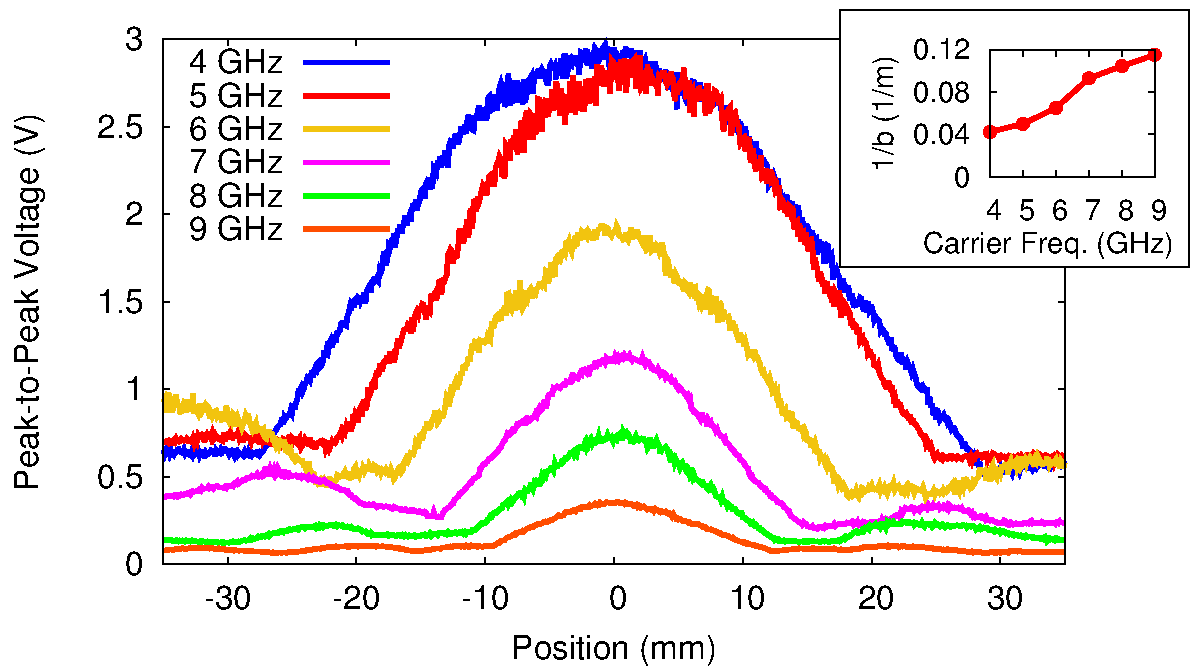
\includegraphics[width=\columnwidth]{spatial/freq_profile.pdf}
\caption[Spatial profile of reconstruction at various frequencies]{Spatial profile of \ptp{} voltage of reconstructions investigated at carrier frequencies ranging from 4 to 9 GHz in 1 GHz
steps.  The inset shows the inverse of the fit $b$ values versus carrier frequency, showing the expected linear relationship.}
\label{fig:spatial-freq-profile}

\vspace*{\floatsep}% http://tex.stackexchange.com/q/26521/5764

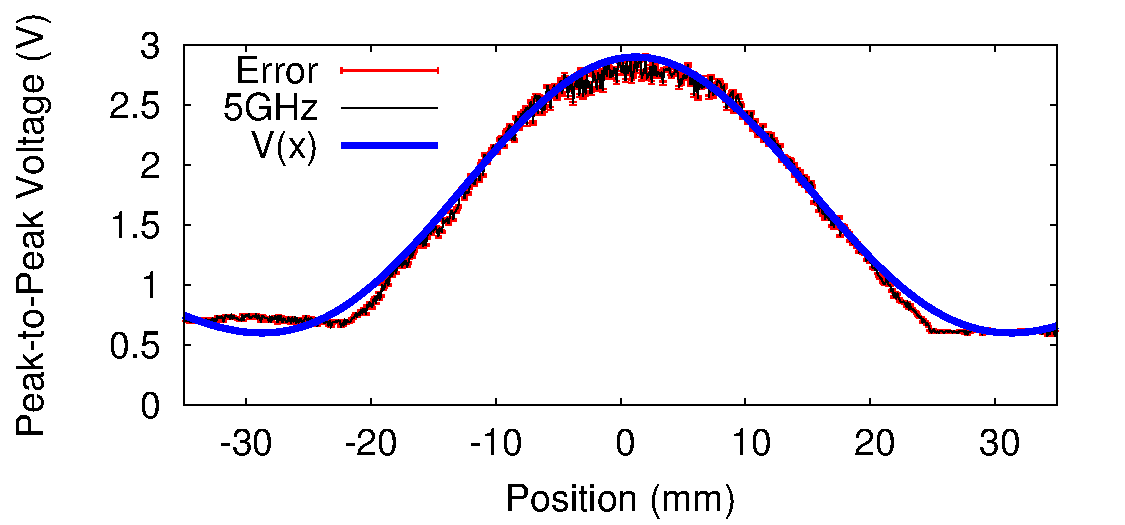
\includegraphics[width=\columnwidth]{spatial/fit.pdf}
\caption[Fit of spatial profile]{Measured \ptp{} voltage of reconstructions received in the
vicinity of a time-reversed wave collapse location with a 5 GHz carrier
frequency, and fit to the \texttt{sinc(x)} function. The parameters here are $a = 2.18 \pm 0.046397869$, $b = 26.72 \pm 0.134629783$, $c = -73.58 \pm 0.116338652$, and $d = 0.43 \pm 0.012711137$. The fit parameters for the remaining 4-9~GHz frequency profiles from Figure~\ref{fig:spatial-freq-profile} are given in Appendix~\ref{app:spatial-fit-params}.}
\label{fig:spatial-error-fit}
\end{figure}

Based on observations from the results in Figure~\ref{fig:spatial-freq-profile}, we expect the reconstruction \ptp{} voltage profile to take the form of a $sinc(x)$ function about the target location~\cite{lerosey-focusing}. Thus, we propose the following equation to predict $V(x)$, the maximum \ptp{} voltage from a given reconstruction, as a function of $x$, the distance between the reconstruction focal point and the receiver:

\begin{equation}
\label{eq:vx}
V(x) = a\cdot sinc\left(\frac{x+c}{b}\right) + d
\end{equation}

where $a$ is the maximum \ptp{} reconstruction amplitude, $b$ is the half-wavelength, $c$ is the location of the antenna along the x-axis, and $d$ is the noise level offset voltage. Since $b$ is proportional to the wavelength (and inversely proportional to frequency), as the carrier frequency is increased,  $\frac{1}{b}$ also increases, causing the ``bubble'' of the sinc function in Figure~\ref{fig:spatial-freq-profile} to get smaller. This relationship is shown explicitly in the inset of Figure~\ref{fig:spatial-freq-profile}. Figure~\ref{fig:spatial-error-fit} shows Equation~\ref{eq:vx} fit to the 5 GHz curve from Figure~\ref{fig:spatial-freq-profile}, including error bars. The fit qualitatively looks good around the main lobe, but quantitatively has a high reduced $\chi^2$ value, primarily due to the rather large background noise level that has hidden the side lobes. Fitting to just the main lobe produces a much better goodness of fit metric. The error bars are primarily systematic, introduced by the oscilloscope internal voltage multiplier used in scaling.

The results presented in Figure~\ref{fig:spatial-freq-profile} allow us to draw several conclusions. In this frequency range, the reconstructions can be categorized as broad, spanning several centimeters in width. This is significant because it indicates that we can move the receiver slightly away from the target location and still collect energy from the reconstruction. This allows us to implement a system targeting a moving receiver.

\subsection{Reconstructing on a Moving Target}
\label{sec:recon-moving}

\subsubsection{Methodology}
For this experiment, the receiving antenna was moved at a constant speed of 0.2~$\frac{mm}{s}$ across the entire 70~mm range provided by the translation stage. To counteract the degradation of reconstruction strength as the antenna moved, we periodically repeated the interrogation step, effectively re-centering the reconstruction on the antenna. Since the test equipment does not allow broadcast of one sona while collecting another, it was not possible to transmit power during the collection time, leading to a finite ``dead time,'' denoted $t_d$ in Figure~\ref{fig:moving-recon}. During the broadcast period, the time-reversed sona was continually broadcast into the cavity (once every 15~$\mu$s) and the peak-to peak voltage across the receiver was measured once every 2.05~seconds, meaning that the reconstructions are highly undersampled in this plot. After every 15 samples were collected, the process was repeated. We refer to this full process of collecting a new sona and then broadcasting it for a given period time as a full ``cycle'' of length $t_c$. The results in Figure~\ref{fig:moving-recon}  below were obtained using a carrier frequency of 5 GHz, $t_d$ of 7 seconds, and $t_c$ of 39.8 seconds. Based on the results from Section~\ref{sec:spatial-results}, the \ptp{} reconstruction voltage measured by the receiver is expected to decay according to the $sinc(x)$ function as the receiver moves away from the reconstruction focal point. This $sinc(x)$ function will be centered on the position where the sona was last collected, making the reconstruction focus continually lag behind the antenna. Consequently, the maximum reconstruction strength is limited by the time needed to collect, time reverse and re-broadcast an updated sona. The following equation is proposed as a model for the \ptp{} voltage of the reconstruction on a moving target as a function of time, assuming a constant velocity $\bar{v}$:

\begin{equation}\label{eq:vt}
%\begin{displaymath}
  V(t) = \left\{
        \begin{array}{ll}
                0 & : t\pmod{t_c} \le t_d \\
                a\cdot sinc(\frac{\bar{v}t}{b})+d & : t\pmod{t_c} > t_d
        \end{array}\,.
  \right.
%\end{displaymath}
\end{equation}

\subsubsection{Results}
\label{moving-results}

The results of this experiment are very promising. We hypothesized that the reconstruction \ptp{} voltage would reset back to a maximal value when a new sona was used to refocus the reconstruction, and follow the voltage profile as the receiver moved away from the new target location. This was almost exactly confirmed by the experimental results. This is encouraging for the application of TR to a practical WPT scheme because it proves the applicability to a moving receiver system.

\begin{figure}[t]
\centering
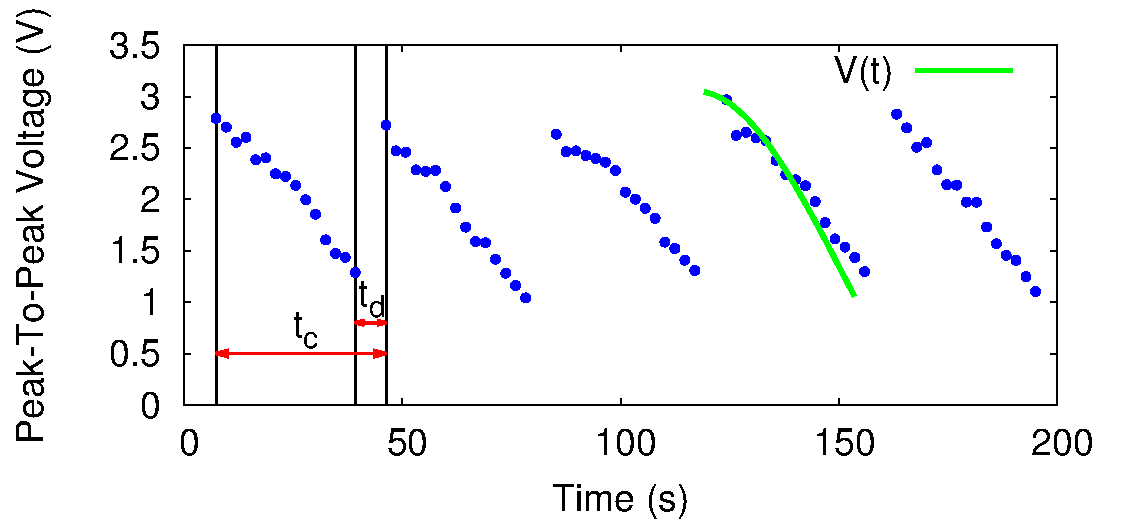
\includegraphics[width=0.85\textwidth]{moving/moving_recon}
    \caption[\Ptp{} voltage of moving reconstructions]{Reconstruction \ptp{} voltage vs. time as the target moves along one wall of the enclosure. A new sona signal is acquired every $t_c = 39.8s$, leading to a dead time of duration $t_d = 7s$. The target is moving at a speed of 0.5~$\frac{mm}{s}$ and the carrier frequency is 5~GHz. The green line is Eq.~\ref{eq:vt}.}
    \label{fig:moving-recon}
\end{figure}

It is worth noting that the speed of the receiver is relatively slow at 0.2~$\frac{mm}{s}$. This experiment is intended to be a proof of concept, with generalized equipment that carries significant overhead. The GPIB connections between the signal generators, oscilloscope, and workstation contributed to the long delay between system operations, in addition to the slow processing speed of the equipment itself. We expect that with a dedicated time reversal system, the TR process of reacquiring a new target location could be performed in milliseconds and describe the ramifications for doing so in Section~\ref{sec:future-timing}. This would greatly increase the maximum receiver speed that could be accommodated as the reconstruction could be refocused more often, and thus the average \ptp{} voltage could be raised closer to that maximal value. We conclude that, with further research and engineering work, a TR WPT scheme could feasibly power a moving receiver in realistic scenarios.
